\documentclass[conference,a4paper,10pt]{IEEEtran}
\IEEEoverridecommandlockouts

\usepackage{cite}
\usepackage{amsmath,amssymb,amsfonts}
\usepackage{algorithmic}
\usepackage{graphicx}
\usepackage{textcomp}
\usepackage{xcolor}
\usepackage{caption}
\usepackage{subcaption}
\usepackage{multirow}
\usepackage{booktabs}
\usepackage{url}
\usepackage[
  left=16mm,
  right=16mm,
  top=19mm,
  bottom=23mm
]{geometry}
\def\BibTeX{{\rm B\kern-.05em{\sc i\kern-.025em b}\kern-.08em
    T\kern-.1667em\lower.7ex\hbox{E}\kern-.125emX}}
\begin{document}

\title{Computer Vision for Ball Detection and Table Rectification in 8-Ball Pool Images}

% \author{
% \IEEEauthorblockN{1\textsuperscript{st} First Author}
% \IEEEauthorblockA{\textit{dept. of Informatics Engineering} \\
% \textit{Faculty of Engineering} \\ \textit{University of Porto}\\ Porto, Portugal \\
% first@up.pt}
% \and
% \IEEEauthorblockN{2\textsuperscript{nd} Second Author}
% \IEEEauthorblockA{\textit{dept. of Informatics Engineering} \\
% \textit{Faculty of Engineering} \\ \textit{University of Porto}\\ Porto, Portugal \\
% second@up.pt}
% }

\author{
\IEEEauthorblockN{Diogo Marques, Mansur Mustafin}
\IEEEauthorblockA{
\textit{Dept. of Informatics Engineering}\\
\textit{Faculty of Engineering of the University of Porto}\\
Porto, Portugal\\
Email: 202008445@fe.up.pt, 202102355@fe.up.pt
}
}


\maketitle

\begin{abstract}
Example of abstract text.
\end{abstract}

\begin{IEEEkeywords}
IEEE; Template; University.
\end{IEEEkeywords}
\section{Introduction}
\label{sec:introduction}

This work presents a computer vision approach for analyzing images of 8-ball pool tables. The system detects the balls, estimates their positions, identifies their numbers, and reconstructs a top-view of the table.

% \section{Related Work}
\label{sec:related_work}

\section{Methods}
\label{sec:methods}

\subsection{Table Localization and Perspective Rectification}

The objective is to convert an image of a pool table into a normalized top-view representation. In addition to removing projective distortion, the method also rotates the rectified table so that the center spot is placed on the right-hand side of the final image. The overall processing pipeline is illustrated in Figure~\ref{fig:topview-pipeline}.

The processing pipeline begins with image normalization. The input image is resized to a fixed width in order to reduce scale variability. A Gaussian blur is then applied before color analysis.

Table localization is performed in the HSV color space using an adaptive estimate of the cloth color. Instead of applying a fixed threshold, the method analyzes a central region of the image, where the table surface is expected to dominate. After excluding pixels with low saturation and low value, the dominant hue is estimated from the corresponding histogram. Dominant saturation and value levels are then determined around this hue.

After thresholding, the resulting binary mask is refined with morphological opening and closing to remove isolated noise and fill small gaps. Because the scene may contain other objects with similar colors, only contours that are spatially close to the largest table-colored region are retained. This step preserves the full table area while discarding unrelated background regions.

The table boundaries are recovered from the cleaned mask through edge detection followed by a probabilistic Hough transform \cite{Canny1986,MATAS2000119}. Only sufficiently long line segments are kept, since short segments are more likely to correspond to noise. Each detected segment is then converted into Hesse normal form, which provides a convenient representation for comparing orientation and distance from the table center. Lines with similar orientation and nearby offsets are grouped together, and within each group the line farther from the center is interpreted as an outer cushion boundary while the closer one is treated as an inner playing-surface boundary.

In challenging cases, more than four candidate line groups may be produced. To obtain a single rectangular hypothesis, combinations of four lines are evaluated by intersecting them and scoring the resulting quadrilateral. The score favors large shapes whose opposite sides have similar lengths, which is consistent with the expected geometry of a billiard table. If the initial color thresholding yields too few valid lines, the hue interval is relaxed and the detection stage is repeated.

Once the four relevant boundaries are selected, the lines are ordered clockwise around the estimated table center and their intersections are used to define the table corners. Two perspective rectifications are then performed \cite{Hartley2004}. First, the inner boundary is warped to a square reference image, which provides a convenient intermediate view for orientation analysis. Second, after the correct orientation has been determined, the outer boundary is warped to the final rectangular top-view image.

From the initial square warp, four small patches are sampled at the right, bottom, left, and top sides of the table. Each patch is examined for non-cloth regions using the previously estimated table color. After morphological cleanup, contour size and contact with the patch border are used to distinguish small cue-position markers from larger regions caused by a ball. The preferred orientation is chosen according to the strongest available cue: a detected marker alone is preferred, followed by a marker accompanied by a ball, and finally by the largest ball-like region. If none of these visual cues is sufficiently reliable, a fallback rule based on the coarse viewpoint geometry of the detected quadrilateral is used.

During perspective warping, some transformed coordinates may fall outside the source image. For this reason, the final top-view includes a small padding margin around the table.

\begin{figure*}[t]
    \centering
    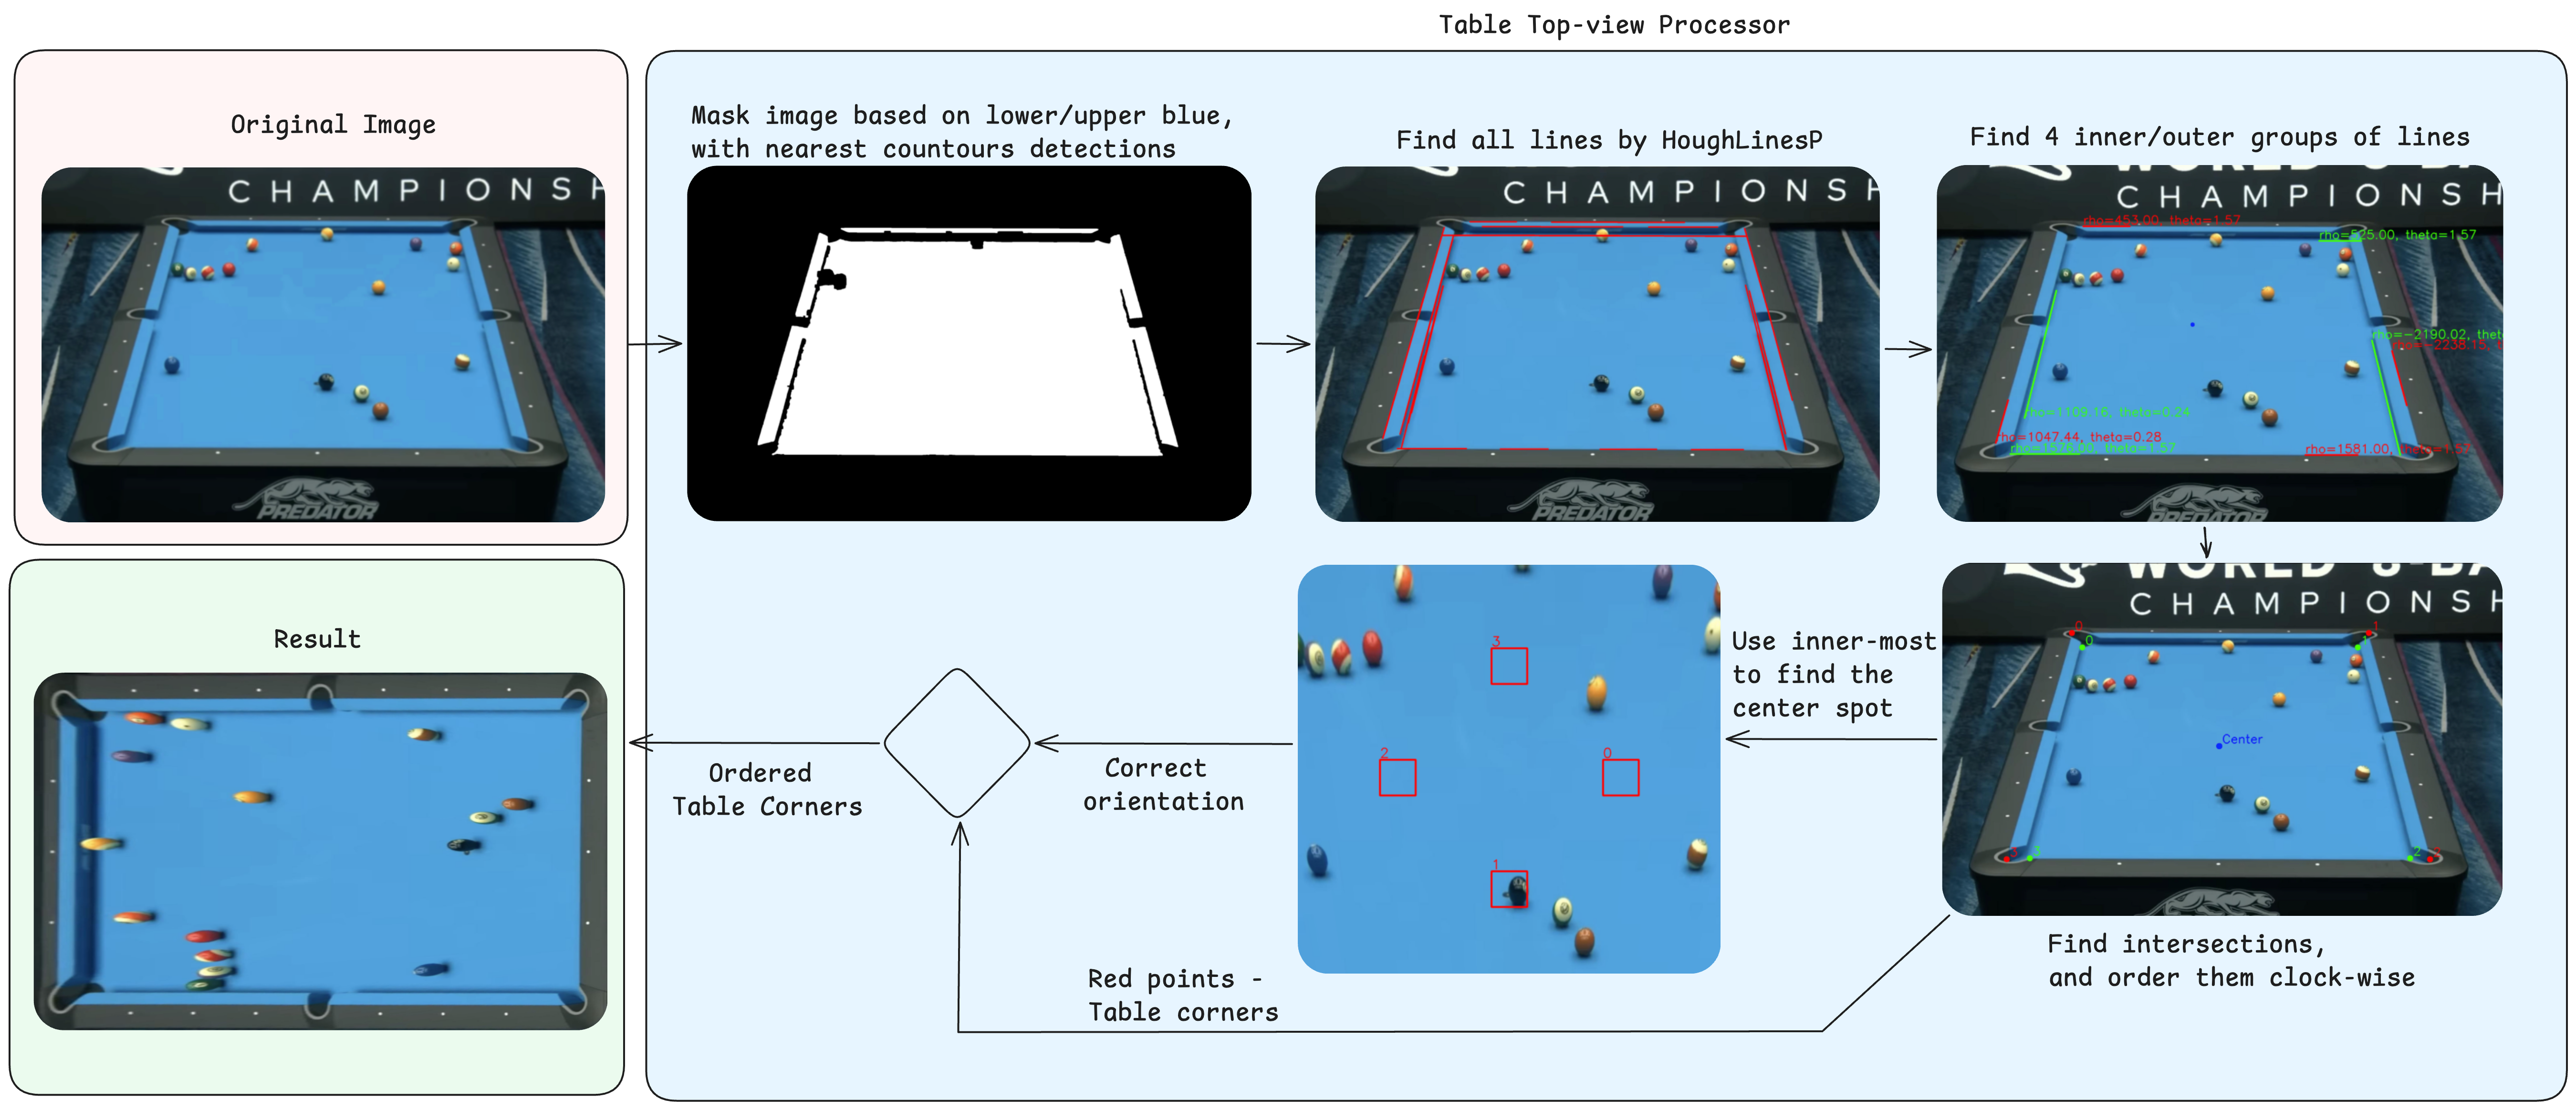
\includegraphics[width=0.95\linewidth]{img/top_view_pipeline.png}
    \caption{Pipeline for table localization, perspective rectification, and orientation normalization.}
    \label{fig:topview-pipeline}
\end{figure*}


\subsection{Ball Position Detection}

\begin{itemize}
    \item Obtain the inner and outer table lines, corner points, and the view angle using the functions described in the previous section.
    
    \item Apply a shadow mask to the boundary regions between the inner and outer lines according to the view angle:
    \begin{itemize}
        \item \textbf{Front view:} apply the mask to the top region.
        \item \textbf{Angled view:} apply the mask to the side regions.
        \item \textbf{Top view:} no mask is applied.
    \end{itemize}
    
    \item Patch holes according to the view angle:
    \begin{itemize}
        \item \textbf{Front or angled view:} patch corner holes using a semicircle centered between the points defined by the intersections of the outer and inner lines, with radius given by the distance between these points.
        \item \textbf{Top view:} since there is no perspective distortion and the holes are larger, use the calculated midpoints and patch them with a circle of fixed radius.
    \end{itemize}
    
    \item Remove the background using the sampled mode of the H, S, and V pixel values, with increased tolerance to eliminate additional shadows beneath and around the balls.
    
    \item Apply dilation followed by erosion using an elliptical $3\times3$ kernel for six iterations.
    
    \item Apply erosion followed by dilation using an elliptical $3\times3$ kernel for six iterations.
    
    \item Apply a median blur with a $7\times7$ kernel.
    
    \item Detect circles using the Hough Circle Transform with parameters fine-tuned for different view angles.
    
    \item Remove overlapping circles and circles whose centers lie outside the inner table lines:
    \begin{itemize}
        \item If
        \[
        A_{\text{small}} < 0.4 \, A_{\text{large}},
        \]
        remove the smaller circle.
        
        \item If
        \[
        \mathrm{area}(C_{\text{small}} \cap C_{\text{large}}) \geq 0.5 \, A_{\text{small}},
        \]
        keep the larger circle.
    \end{itemize}
\end{itemize}

\begin{figure}[h]
    \centering
    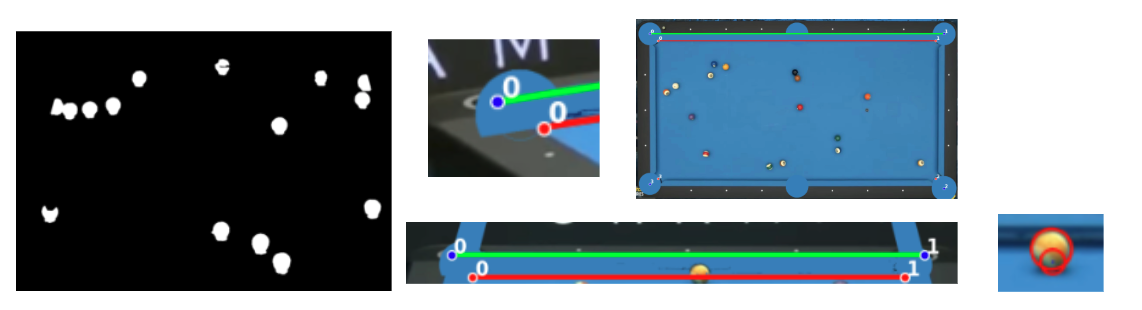
\includegraphics[width=\linewidth]{img/ball_position_detection.png}
    \caption{Left: final color mask. Middle: effect of patching holes and removing shadows. Right: removal of overlapping circles.}
    \label{fig:ball_position_detection}
\end{figure}

\subsection{Ball Number (Color) Detection}

\begin{itemize}
    \item Calibrate the reference colors by sampling the balls on the table.
    
    \item \textbf{White and black balls:} threshold the percentage of pixels identified as black or white, and assign the label to the ball with the highest percentage.
    
    \item \textbf{Striped or solid balls:} classify them using the percentage of white pixels.
    
    \item Initialize a dictionary of the form
    \[
    C_1, \ldots, C_n : b_1, \ldots, b_m,
    \]
    where $n$ is the total number of colors and $m$ is the number of balls on the table. Each entry stores the distance of every ball to the corresponding reference color in RGB space.
    
    \item Convert this dictionary into a definite assignment map using either:
    \begin{itemize}
        \item a greedy approach, in which the smallest distance between any ball and any color is repeatedly selected until every color has at least one associated ball, or
        \item the Hungarian algorithm, which minimizes the total assignment cost (see Annex~I).
    \end{itemize}
    
    \item For each detected ball, check the assignment map and assign the most probable color (number).
\end{itemize}

\section{Results}
\label{sec:results}

The generated top-view images produced good results in most cases, providing a stable and visually consistent representation of the table. Their correctness was assessed manually by checking whether the resulting image was geometrically and orientation-wise correct.

% \section{Conclusion}
\label{sec:conclusion}


\bibliographystyle{IEEEtran}
\bibliography{refs}

\end{document}
